\documentclass{beamer}

\usefonttheme{professionalfonts} % using non standard fonts for beamer
\usefonttheme{serif} % default family is serif

\usepackage{hyperref}
%\usepackage{minted}
\usepackage{animate}
\usepackage{graphicx}
\def\Put(#1,#2)#3{\leavevmode\makebox(0,0){\put(#1,#2){#3}}}
\usepackage{color}
\usepackage{tikz}
\usepackage{amssymb}
\usepackage{enumerate}


\newcommand\blfootnote[1]{%

  \begingroup

  \renewcommand\thefootnote{}\footnote{#1}%

  \addtocounter{footnote}{-1}%

  \endgroup

}

\makeatletter

%%%%%%%%%%%%%%%%%%%%%%%%%%%%%% Textclass specific LaTeX commands.

 % this default might be overridden by plain title style

 \newcommand\makebeamertitle{\frame{\maketitle}}%

 % (ERT) argument for the TOC

 \AtBeginDocument{%

   \let\origtableofcontents=\tableofcontents

   \def\tableofcontents{\@ifnextchar[{\origtableofcontents}{\gobbletableofcontents}}

   \def\gobbletableofcontents#1{\origtableofcontents}

 }

%%%%%%%%%%%%%%%%%%%%%%%%%%%%%% User specified LaTeX commands.

\usetheme{Malmoe}

% or ...

\useoutertheme{infolines}

\addtobeamertemplate{headline}{}{\vskip2pt}

\setbeamercovered{transparent}

% or whatever (possibly just delete it)

\makeatother

\begin{document}
\title[PFLOCK report]{PFLOCK Report}
\author[AC]{Andres Calderon}
\institute[Fall'19]{University of California, Riverside}
\makebeamertitle
\newif\iflattersubsect

\AtBeginSection[] {
    \begin{frame}<beamer>
    \frametitle{Outline} 
    \tableofcontents[currentsection]  
    \end{frame}
    \lattersubsectfalse
}

\AtBeginSubsection[] {
    \begin{frame}<beamer>
    \frametitle{Outline} 
    \tableofcontents[currentsubsection]  
    \end{frame}
}

\begin{frame}{Working on Brinkhoff dataset}
    \begin{itemize}
        \item Run experiments with the original dataset.
        \item Setting parameters according to paper:  
        \begin{itemize}
            \item Epsilon[m]: 3.77, 7.55 and 11.33
            \item Width[m]: 300
        \end{itemize}
        \item Running on Cluser (10 nodes, 12 cores each) and Standalone (1 core)
        \item Collect execution time for GRIndex and DBScan stages.
    \end{itemize}
\end{frame}

\begin{frame}{Performing experiments in Brinkhoff dataset}
    {\small Cluster: 500 Time instants.}
    \centering
    \begin{minipage}{.5\textwidth}
        \begin{figure}
            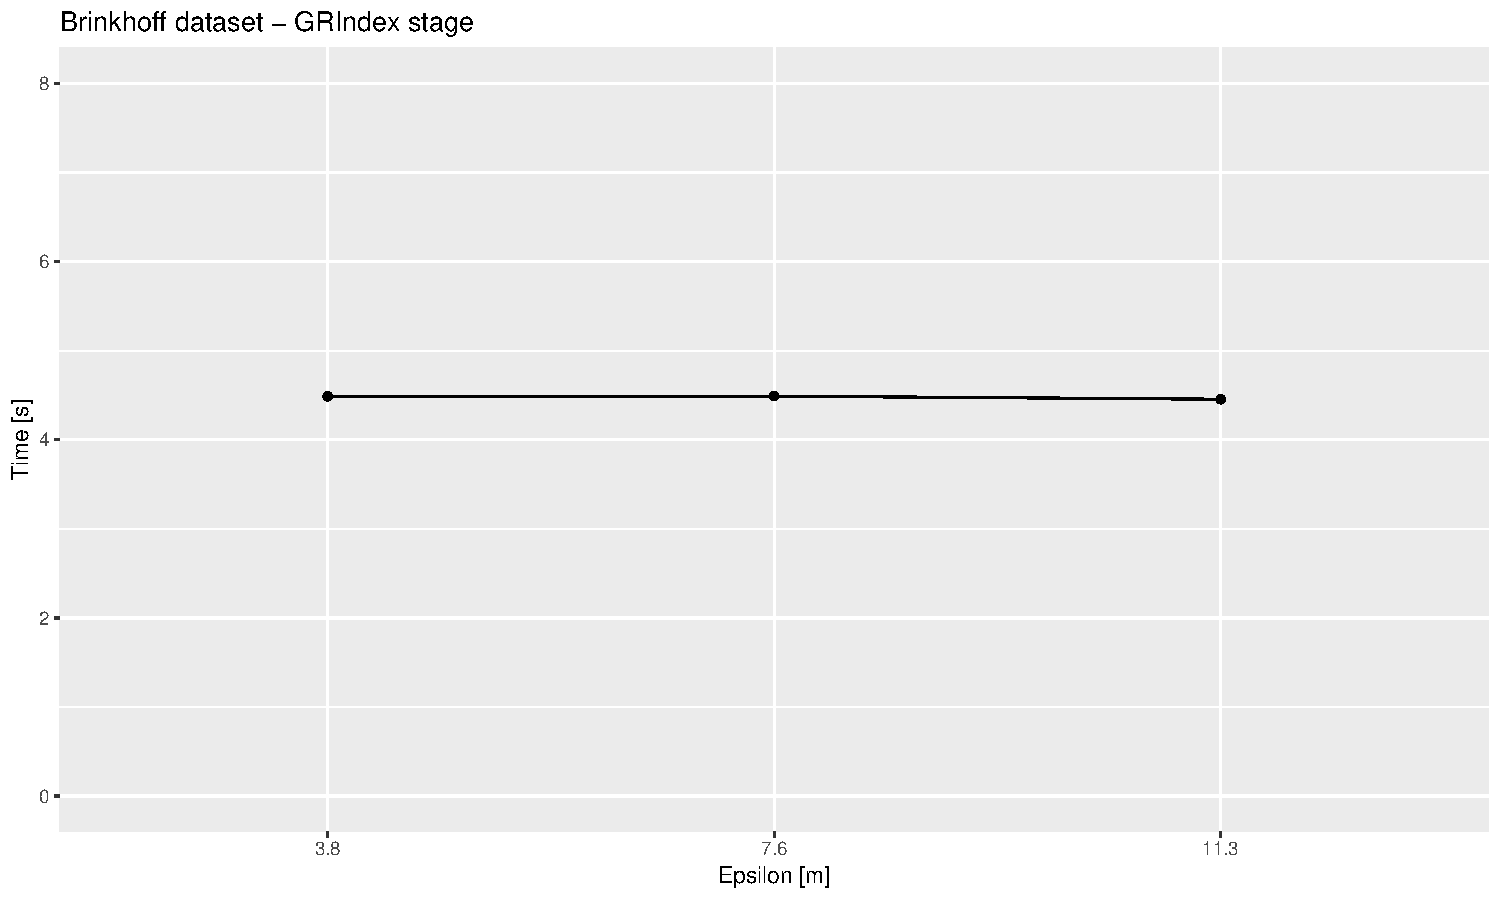
\includegraphics[width=\textwidth]{ICPETesterClusterGRIndex}
        \end{figure}   
    \end{minipage}% This must go next to `\end{minipage}`
    \begin{minipage}{.5\textwidth}
        \begin{figure}
            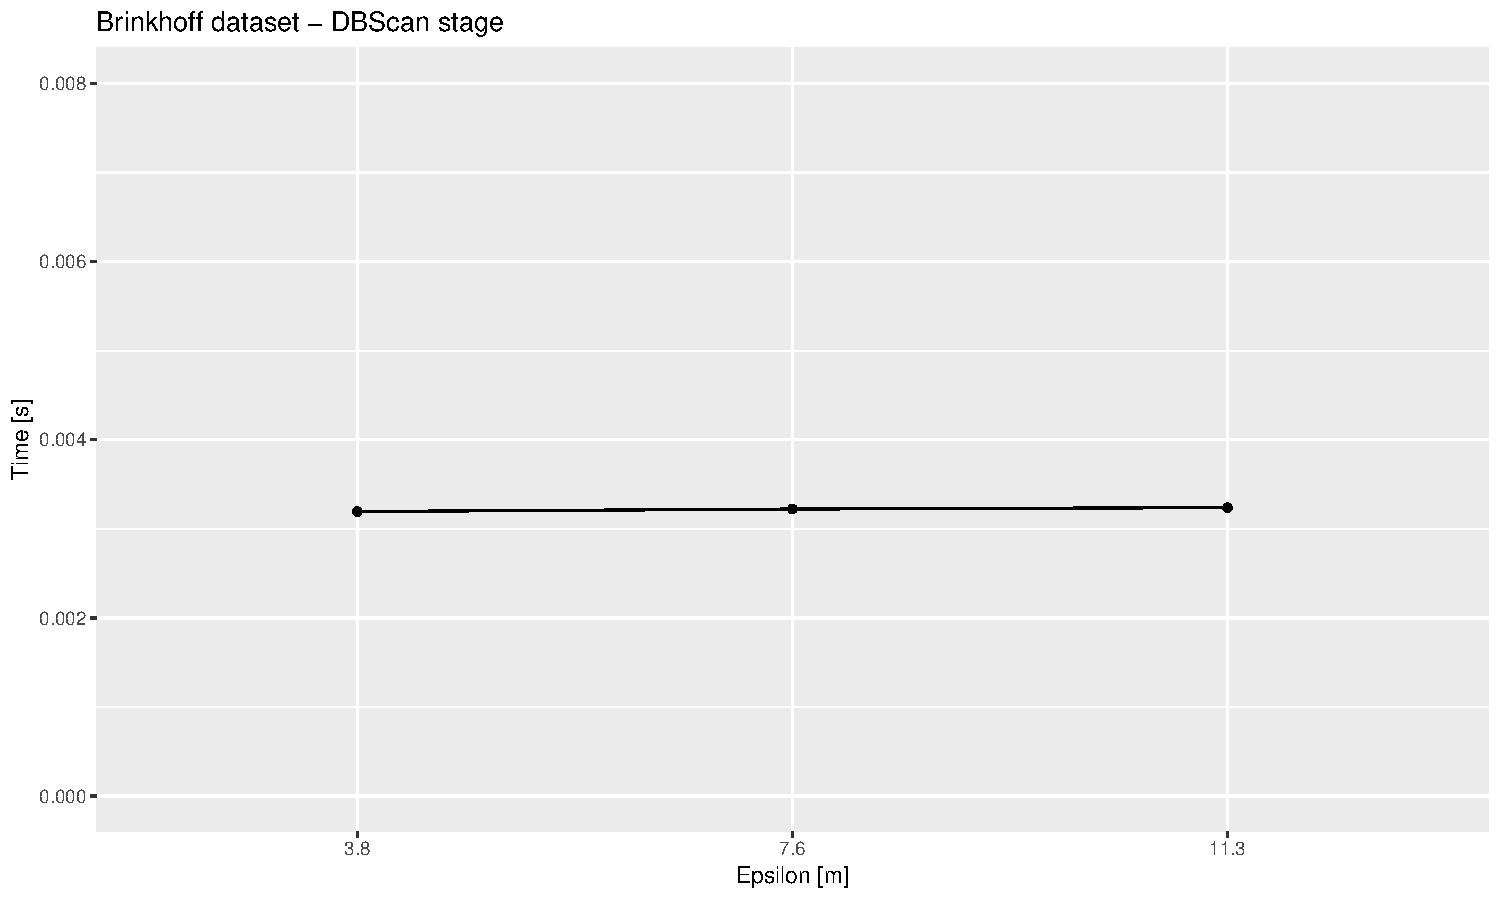
\includegraphics[width=\textwidth]{ICPETesterClusterDBScan}
        \end{figure}   
    \end{minipage}
\end{frame}

\begin{frame}{Performing experiments in Brinkhoff dataset}
    {\small Standalone: 100 Time instants.}
    \centering
    \begin{minipage}{.5\textwidth}
        \begin{figure}
            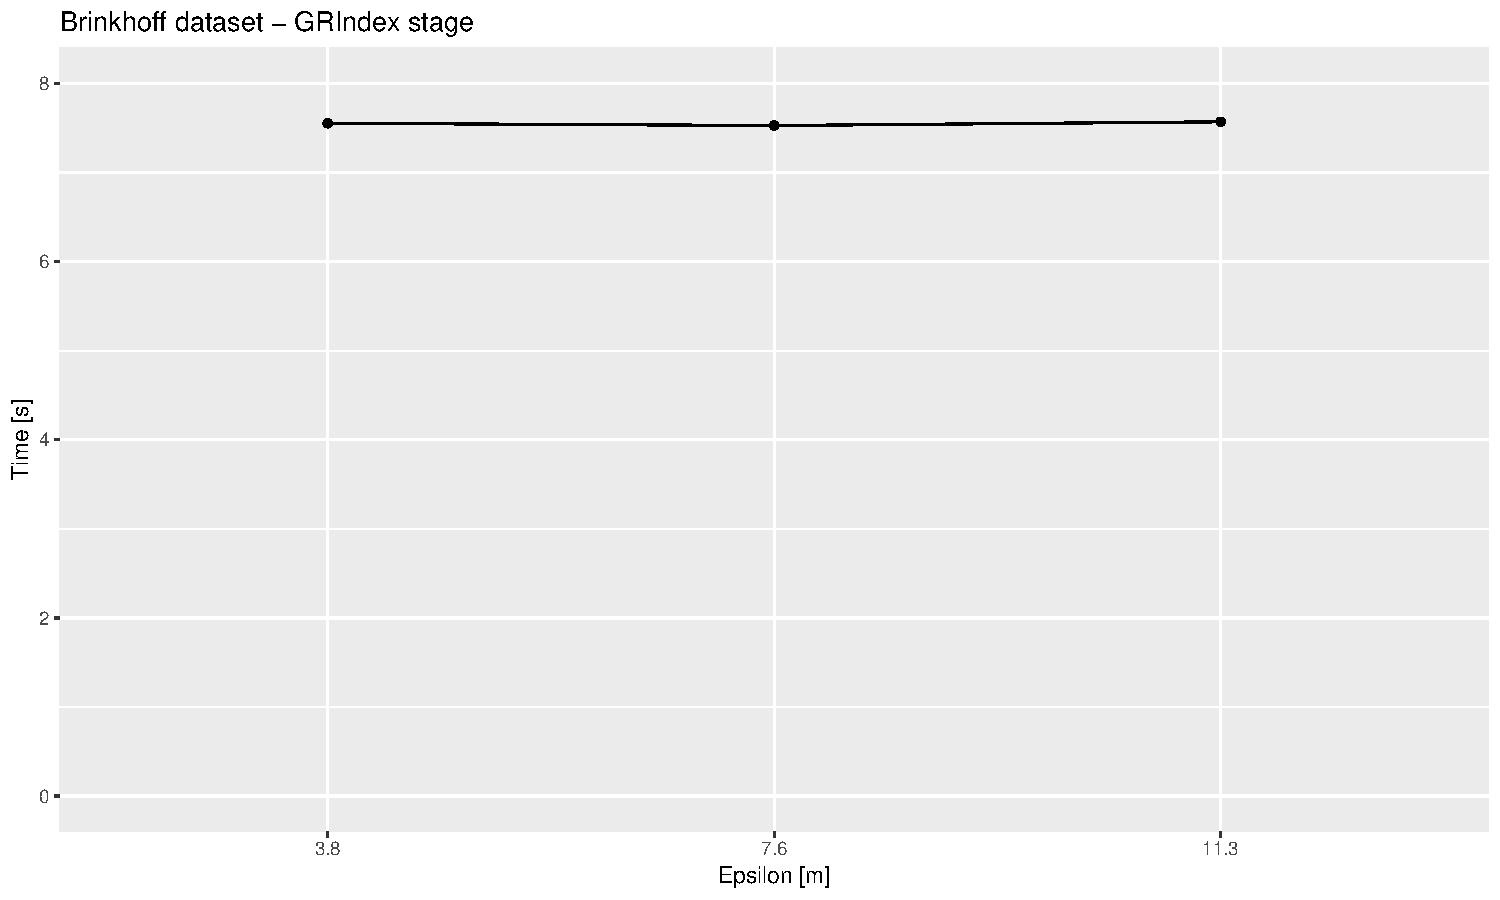
\includegraphics[width=\textwidth]{ICPETesterStandaloneGRIndex}
        \end{figure}   
    \end{minipage}% This must go next to `\end{minipage}`
    \begin{minipage}{.5\textwidth}
        \begin{figure}
            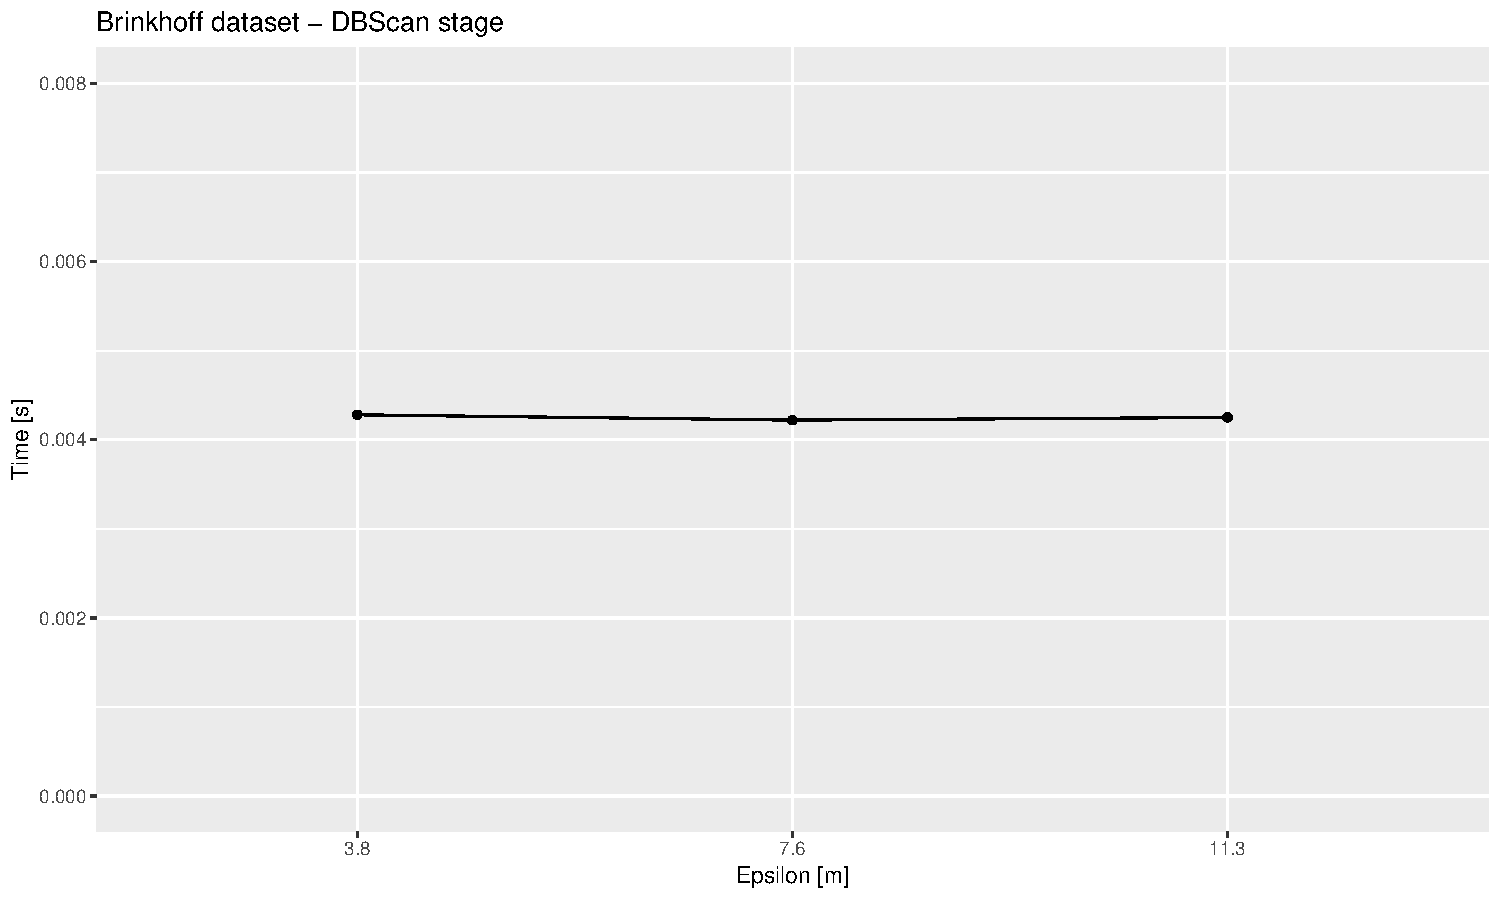
\includegraphics[width=\textwidth]{ICPETesterStandaloneDBScan}
        \end{figure}   
    \end{minipage}
\end{frame}

\begin{frame}{Fixed Length Bit Compression method}
    \begin{itemize}
        \item I have solved the issue with the streaming environment, but I would like to talk about the rate of data ingestion.
        \item I have finished the implementation in order to find flocks.  Tests with dummy data are ok.
    \end{itemize}
\end{frame}


\begin{frame}{What is next?}
    \begin{itemize}
        \item Integrate Fixed Length Bit Compression method with the GRIndex routine and our implementation.
        \item Run experiments with LA\_25K and LA\_50K. (Alternatively GeoSparkSim\footnote{\url{http://www.public.asu.edu/~jiayu2/geospark/publication/geosparksim-mdm-2019.pdf}}).  
        \item Explore suitable real datasets (NYTaxis, eBirds).
    \end{itemize}
\end{frame}

\end{document}
